\documentclass[twoside]{book}

% Packages required by doxygen
\usepackage{fixltx2e}
\usepackage{calc}
\usepackage{doxygen}
\usepackage[export]{adjustbox} % also loads graphicx
\usepackage{graphicx}
\usepackage[utf8]{inputenc}
\usepackage{makeidx}
\usepackage{multicol}
\usepackage{multirow}
\PassOptionsToPackage{warn}{textcomp}
\usepackage{textcomp}
\usepackage[nointegrals]{wasysym}
\usepackage[table]{xcolor}

% Font selection
\usepackage[T1]{fontenc}
\usepackage[scaled=.90]{helvet}
\usepackage{courier}
\usepackage{amssymb}
\usepackage{sectsty}
\renewcommand{\familydefault}{\sfdefault}
\allsectionsfont{%
  \fontseries{bc}\selectfont%
  \color{darkgray}%
}
\renewcommand{\DoxyLabelFont}{%
  \fontseries{bc}\selectfont%
  \color{darkgray}%
}
\newcommand{\+}{\discretionary{\mbox{\scriptsize$\hookleftarrow$}}{}{}}

% Page & text layout
\usepackage{geometry}
\geometry{%
  a4paper,%
  top=2.5cm,%
  bottom=2.5cm,%
  left=2.5cm,%
  right=2.5cm%
}
\tolerance=750
\hfuzz=15pt
\hbadness=750
\setlength{\emergencystretch}{15pt}
\setlength{\parindent}{0cm}
\setlength{\parskip}{0.2cm}
\makeatletter
\renewcommand{\paragraph}{%
  \@startsection{paragraph}{4}{0ex}{-1.0ex}{1.0ex}{%
    \normalfont\normalsize\bfseries\SS@parafont%
  }%
}
\renewcommand{\subparagraph}{%
  \@startsection{subparagraph}{5}{0ex}{-1.0ex}{1.0ex}{%
    \normalfont\normalsize\bfseries\SS@subparafont%
  }%
}
\makeatother

% Headers & footers
\usepackage{fancyhdr}
\pagestyle{fancyplain}
\fancyhead[LE]{\fancyplain{}{\bfseries\thepage}}
\fancyhead[CE]{\fancyplain{}{}}
\fancyhead[RE]{\fancyplain{}{\bfseries\leftmark}}
\fancyhead[LO]{\fancyplain{}{\bfseries\rightmark}}
\fancyhead[CO]{\fancyplain{}{}}
\fancyhead[RO]{\fancyplain{}{\bfseries\thepage}}
\fancyfoot[LE]{\fancyplain{}{}}
\fancyfoot[CE]{\fancyplain{}{}}
\fancyfoot[RE]{\fancyplain{}{\bfseries\scriptsize Generated on Sun Dec 6 2015 14\+:06\+:30 for C\+S294-\/73 Final Project of Group H\+: Dendritic Growth by Doxygen }}
\fancyfoot[LO]{\fancyplain{}{\bfseries\scriptsize Generated on Sun Dec 6 2015 14\+:06\+:30 for C\+S294-\/73 Final Project of Group H\+: Dendritic Growth by Doxygen }}
\fancyfoot[CO]{\fancyplain{}{}}
\fancyfoot[RO]{\fancyplain{}{}}
\renewcommand{\footrulewidth}{0.4pt}
\renewcommand{\chaptermark}[1]{%
  \markboth{#1}{}%
}
\renewcommand{\sectionmark}[1]{%
  \markright{\thesection\ #1}%
}

% Indices & bibliography
\usepackage{natbib}
\usepackage[titles]{tocloft}
\setcounter{tocdepth}{3}
\setcounter{secnumdepth}{5}
\makeindex

% Hyperlinks (required, but should be loaded last)
\usepackage{ifpdf}
\ifpdf
  \usepackage[pdftex,pagebackref=true]{hyperref}
\else
  \usepackage[ps2pdf,pagebackref=true]{hyperref}
\fi
\hypersetup{%
  colorlinks=true,%
  linkcolor=blue,%
  citecolor=blue,%
  unicode%
}

% Custom commands
\newcommand{\clearemptydoublepage}{%
  \newpage{\pagestyle{empty}\cleardoublepage}%
}


%===== C O N T E N T S =====

\begin{document}

% Titlepage & ToC
\hypersetup{pageanchor=false,
             bookmarks=true,
             bookmarksnumbered=true,
             pdfencoding=unicode
            }
\pagenumbering{roman}
\begin{titlepage}
\vspace*{7cm}
\begin{center}%
{\Large C\+S294-\/73 Final Project of Group H\+: Dendritic Growth }\\
\vspace*{1cm}
{\large Generated by Doxygen 1.8.10}\\
\vspace*{0.5cm}
{\small Sun Dec 6 2015 14:06:30}\\
\end{center}
\end{titlepage}
\clearemptydoublepage
\tableofcontents
\clearemptydoublepage
\pagenumbering{arabic}
\hypersetup{pageanchor=true}

%--- Begin generated contents ---
\chapter{Class Index}
\section{Class List}
Here are the classes, structs, unions and interfaces with brief descriptions\+:\begin{DoxyCompactList}
\item\contentsline{section}{\hyperlink{classAutoStart}{Auto\+Start} }{\pageref{classAutoStart}}{}
\item\contentsline{section}{\hyperlink{classAutoStartLeaf}{Auto\+Start\+Leaf} }{\pageref{classAutoStartLeaf}}{}
\item\contentsline{section}{\hyperlink{classBox}{Box} }{\pageref{classBox}}{}
\item\contentsline{section}{\hyperlink{classDendritic}{Dendritic} }{\pageref{classDendritic}}{}
\item\contentsline{section}{\hyperlink{classDendriticGrowth}{Dendritic\+Growth} }{\pageref{classDendriticGrowth}}{}
\item\contentsline{section}{\hyperlink{classDendriticShift}{Dendritic\+Shift} }{\pageref{classDendriticShift}}{}
\item\contentsline{section}{\hyperlink{structelem}{elem} }{\pageref{structelem}}{}
\item\contentsline{section}{\hyperlink{classPoint}{Point} }{\pageref{classPoint}}{}
\item\contentsline{section}{\hyperlink{classRectMDArray}{Rect\+M\+D\+Array$<$ T $>$} }{\pageref{classRectMDArray}}{}
\item\contentsline{section}{\hyperlink{classRectMDOperators}{Rect\+M\+D\+Operators} \\*This class is a set of operators that act on \hyperlink{classRectMDArray}{Rect\+M\+D\+Array} and a given point. All of the operators are dimension independent }{\pageref{classRectMDOperators}}{}
\item\contentsline{section}{\hyperlink{classRK4}{R\+K4$<$ X, F, d\+X $>$} \\*Generic explicit \hyperlink{classRK4}{R\+K4} algorithm }{\pageref{classRK4}}{}
\item\contentsline{section}{\hyperlink{classTraceTimer}{Trace\+Timer} }{\pageref{classTraceTimer}}{}
\end{DoxyCompactList}

\chapter{Class Documentation}
\hypertarget{classAutoStart}{}\section{Auto\+Start Class Reference}
\label{classAutoStart}\index{Auto\+Start@{Auto\+Start}}
\subsection*{Public Member Functions}
\begin{DoxyCompactItemize}
\item 
\hypertarget{classAutoStart_a9e0816a258371fe0ec3ea3c14267ef5c}{}{\bfseries Auto\+Start} (\hyperlink{classTraceTimer}{Trace\+Timer} $\ast$a\+\_\+timer, char $\ast$mutex, char $\ast$child\+Mutex)\label{classAutoStart_a9e0816a258371fe0ec3ea3c14267ef5c}

\item 
\hypertarget{classAutoStart_aa3bd9f51f4f29c99c2147903cc6db7d2}{}{\bfseries Auto\+Start} (\hyperlink{classTraceTimer}{Trace\+Timer} $\ast$a\+\_\+timer, char $\ast$mutex)\label{classAutoStart_aa3bd9f51f4f29c99c2147903cc6db7d2}

\item 
\hypertarget{classAutoStart_a391135bddc96b9bda90d46711329fb29}{}bool {\bfseries active} ()\label{classAutoStart_a391135bddc96b9bda90d46711329fb29}

\end{DoxyCompactItemize}


The documentation for this class was generated from the following files\+:\begin{DoxyCompactItemize}
\item 
/home/xingjie/\+Documents/grad\+School/courses/software\+Eng\+For\+Sci\+Comp/final\+Project/github\+Repo/\+C\+S294-\/73/code/src/\+Timer/C\+H\+\_\+\+Timer.\+H\item 
/home/xingjie/\+Documents/grad\+School/courses/software\+Eng\+For\+Sci\+Comp/final\+Project/github\+Repo/\+C\+S294-\/73/code/src/\+Timer/C\+H\+\_\+\+Timer.\+cpp\end{DoxyCompactItemize}

\hypertarget{classAutoStartLeaf}{}\section{Auto\+Start\+Leaf Class Reference}
\label{classAutoStartLeaf}\index{Auto\+Start\+Leaf@{Auto\+Start\+Leaf}}
\subsection*{Public Member Functions}
\begin{DoxyCompactItemize}
\item 
\hypertarget{classAutoStartLeaf_ad31126dbec37c0245fd08bb77be1612b}{}{\bfseries Auto\+Start\+Leaf} (\hyperlink{classTraceTimer}{Trace\+Timer} $\ast$a\+\_\+timer)\label{classAutoStartLeaf_ad31126dbec37c0245fd08bb77be1612b}

\item 
\hypertarget{classAutoStartLeaf_ac6ebea5f14cfea49095514d89f107691}{}bool {\bfseries active} ()\label{classAutoStartLeaf_ac6ebea5f14cfea49095514d89f107691}

\end{DoxyCompactItemize}


The documentation for this class was generated from the following files\+:\begin{DoxyCompactItemize}
\item 
/home/xingjie/\+Documents/grad\+School/courses/software\+Eng\+For\+Sci\+Comp/final\+Project/github\+Repo/\+C\+S294-\/73/code/src/\+Timer/C\+H\+\_\+\+Timer.\+H\item 
/home/xingjie/\+Documents/grad\+School/courses/software\+Eng\+For\+Sci\+Comp/final\+Project/github\+Repo/\+C\+S294-\/73/code/src/\+Timer/C\+H\+\_\+\+Timer.\+cpp\end{DoxyCompactItemize}

\hypertarget{classBox}{}\section{Box Class Reference}
\label{classBox}\index{Box@{Box}}
\subsection*{Public Member Functions}
\begin{DoxyCompactItemize}
\item 
\hypertarget{classBox_a2b61d9eaf29e8f8aa2d29d89a19c6b7c}{}\hyperlink{classBox_a2b61d9eaf29e8f8aa2d29d89a19c6b7c}{Box} (const \hyperlink{classPoint}{Point} \&a\+\_\+low\+Corner, const \hyperlink{classPoint}{Point} \&a\+\_\+high\+Corner)\label{classBox_a2b61d9eaf29e8f8aa2d29d89a19c6b7c}

\begin{DoxyCompactList}\small\item\em constructor for nontrivial \hyperlink{classBox}{Box}. \end{DoxyCompactList}\item 
\hypertarget{classBox_a54f52432a78be9bd16c396da95496798}{}\hyperlink{classBox_a54f52432a78be9bd16c396da95496798}{Box} (const \hyperlink{classBox}{Box} \&a\+\_\+\+Box)\label{classBox_a54f52432a78be9bd16c396da95496798}

\begin{DoxyCompactList}\small\item\em copy constructor. \end{DoxyCompactList}\item 
\hypertarget{classBox_aa636abea0cb64dbbeab47ffd659ddd2f}{}\hyperlink{classBox}{Box} \hyperlink{classBox_aa636abea0cb64dbbeab47ffd659ddd2f}{operator$\ast$} (const \hyperlink{classBox}{Box} \&a\+\_\+right\+Box) const \label{classBox_aa636abea0cb64dbbeab47ffd659ddd2f}

\begin{DoxyCompactList}\small\item\em Computes the intersection of the \hyperlink{classBox}{Box} with right\+Box. \end{DoxyCompactList}\item 
\hypertarget{classBox_a366054107f5e2d32836b8b666e10a3e2}{}\hyperlink{classBox}{Box} \hyperlink{classBox_a366054107f5e2d32836b8b666e10a3e2}{shift} (int a\+\_\+direction, int a\+\_\+offset)\label{classBox_a366054107f5e2d32836b8b666e10a3e2}

\begin{DoxyCompactList}\small\item\em Computes shifted \hyperlink{classBox}{Box} by a\+\_\+offset in direction a\+\_\+direction. \end{DoxyCompactList}\item 
\hypertarget{classBox_a510ddbb4442c8dc1801c5e4d5a3c6cd0}{}\hyperlink{classBox}{Box} \hyperlink{classBox_a510ddbb4442c8dc1801c5e4d5a3c6cd0}{shift} (const \hyperlink{classPoint}{Point} \&a\+\_\+pt)\label{classBox_a510ddbb4442c8dc1801c5e4d5a3c6cd0}

\begin{DoxyCompactList}\small\item\em Computes shifted \hyperlink{classBox}{Box} by a\+\_\+pt. \end{DoxyCompactList}\item 
\hypertarget{classBox_ae55bf559ec09e3968c69210e224789ce}{}\hyperlink{classBox}{Box} \hyperlink{classBox_ae55bf559ec09e3968c69210e224789ce}{grow} (int a\+\_\+numpoints)\label{classBox_ae55bf559ec09e3968c69210e224789ce}

\begin{DoxyCompactList}\small\item\em Grow in all of the coordinate directions by a\+\_\+numpoints. \end{DoxyCompactList}\item 
\hypertarget{classBox_a5e36dea04f5a69f195408a6d0e0592ba}{}\hyperlink{classBox}{Box} \hyperlink{classBox_a5e36dea04f5a69f195408a6d0e0592ba}{grow} (const \hyperlink{classPoint}{Point} \&a\+\_\+pt)\label{classBox_a5e36dea04f5a69f195408a6d0e0592ba}

\begin{DoxyCompactList}\small\item\em Grow in each coordinate direction by an amount given by the component of a\+\_\+pt. \end{DoxyCompactList}\item 
\hypertarget{classBox_acdae3f12a6523dfff88b3cc421b3f675}{}\hyperlink{classBox}{Box} \hyperlink{classBox_acdae3f12a6523dfff88b3cc421b3f675}{coarsen} (int a\+\_\+numpoints)\label{classBox_acdae3f12a6523dfff88b3cc421b3f675}

\begin{DoxyCompactList}\small\item\em coarsen in all of the coordinate directions by a\+\_\+numpoints. \end{DoxyCompactList}\item 
\hypertarget{classBox_ab8edbeddfbefdaccb8f69894cea8d920}{}\hyperlink{classBox}{Box} \hyperlink{classBox_ab8edbeddfbefdaccb8f69894cea8d920}{coarsen} (const \hyperlink{classPoint}{Point} \&a\+\_\+pt)\label{classBox_ab8edbeddfbefdaccb8f69894cea8d920}

\begin{DoxyCompactList}\small\item\em coarsen in each coordinate direction by an amount given by the component of a\+\_\+pt. \end{DoxyCompactList}\item 
\hypertarget{classBox_a0062584dbed1587ad9a8d15425f55055}{}\hyperlink{classBox}{Box} \hyperlink{classBox_a0062584dbed1587ad9a8d15425f55055}{refine} (int a\+\_\+numpoints)\label{classBox_a0062584dbed1587ad9a8d15425f55055}

\begin{DoxyCompactList}\small\item\em refine in all of the coordinate directions by a\+\_\+numpoints. \end{DoxyCompactList}\item 
\hypertarget{classBox_a967c3dbf4d1b64d9100d2f276f967209}{}\hyperlink{classBox}{Box} \hyperlink{classBox_a967c3dbf4d1b64d9100d2f276f967209}{refine} (const \hyperlink{classPoint}{Point} \&a\+\_\+pt)\label{classBox_a967c3dbf4d1b64d9100d2f276f967209}

\begin{DoxyCompactList}\small\item\em refine in each coordinate direction by an amount given by the component of a\+\_\+pt. \end{DoxyCompactList}\item 
\hypertarget{classBox_a1921ede43e51da40e088145e714cd648}{}const \hyperlink{classPoint}{Point} \& \hyperlink{classBox_a1921ede43e51da40e088145e714cd648}{get\+Low\+Corner} () const \label{classBox_a1921ede43e51da40e088145e714cd648}

\begin{DoxyCompactList}\small\item\em Access functions for low, high bounds of \hyperlink{classBox}{Box}. \end{DoxyCompactList}\item 
\hypertarget{classBox_aab4951e1653eeee8086450863154f32b}{}const \hyperlink{classPoint}{Point} \& {\bfseries get\+High\+Corner} () const \label{classBox_aab4951e1653eeee8086450863154f32b}

\item 
\hypertarget{classBox_a13b7df477ab93b4fe974a5151a6c2196}{}int \hyperlink{classBox_a13b7df477ab93b4fe974a5151a6c2196}{linear\+Index} (const \hyperlink{classPoint}{Point} \&a\+\_\+pt) const \label{classBox_a13b7df477ab93b4fe974a5151a6c2196}

\begin{DoxyCompactList}\small\item\em Computes a linear index corresponding to the input array. \end{DoxyCompactList}\item 
\hypertarget{classBox_a18e496a4a686a834850b5d9720a1c322}{}const int \& \hyperlink{classBox_a18e496a4a686a834850b5d9720a1c322}{size\+Of} () const \label{classBox_a18e496a4a686a834850b5d9720a1c322}

\begin{DoxyCompactList}\small\item\em Computes the size of the \hyperlink{classBox}{Box}. \end{DoxyCompactList}\item 
\hypertarget{classBox_a342008fa11641f5b3b79841692411d44}{}bool \hyperlink{classBox_a342008fa11641f5b3b79841692411d44}{operator==} (const \hyperlink{classBox}{Box} \&a\+\_\+rhs\+Box) const \label{classBox_a342008fa11641f5b3b79841692411d44}

\begin{DoxyCompactList}\small\item\em When are two boxes equal. \end{DoxyCompactList}\item 
\hypertarget{classBox_a5af922c141c83b2bb25e522899da5ad5}{}bool \hyperlink{classBox_a5af922c141c83b2bb25e522899da5ad5}{contains} (const \hyperlink{classPoint}{Point} \&a\+\_\+pt) const \label{classBox_a5af922c141c83b2bb25e522899da5ad5}

\begin{DoxyCompactList}\small\item\em Contains the \hyperlink{classPoint}{Point} a\+\_\+pt. \end{DoxyCompactList}\item 
\hypertarget{classBox_a9eb58cb9f4896baa991de834c050d97a}{}int \hyperlink{classBox_a9eb58cb9f4896baa991de834c050d97a}{get\+Index} (const \hyperlink{classPoint}{Point} \&a\+\_\+pt) const \label{classBox_a9eb58cb9f4896baa991de834c050d97a}

\begin{DoxyCompactList}\small\item\em Get linear index of a \hyperlink{classPoint}{Point} in a \hyperlink{classBox}{Box}. \end{DoxyCompactList}\item 
\hypertarget{classBox_a27c222260017eba46f720d8bc2b94b7f}{}bool \hyperlink{classBox_a27c222260017eba46f720d8bc2b94b7f}{not\+Done} (const \hyperlink{classPoint}{Point} \&a\+\_\+pt) const \label{classBox_a27c222260017eba46f720d8bc2b94b7f}

\begin{DoxyCompactList}\small\item\em Says that you have not yet iterated through all ofthe points of the \hyperlink{classBox}{Box}. \end{DoxyCompactList}\item 
void \hyperlink{classBox_a450ac265f84723771d2281785d51d424}{increment} (\hyperlink{classPoint}{Point} \&a\+\_\+pt) const 
\item 
\hypertarget{classBox_a30c40f4155427e7f68704e7607b8de89}{}\hyperlink{classPoint}{Point} \hyperlink{classBox_a30c40f4155427e7f68704e7607b8de89}{get\+Point} (int k) const \label{classBox_a30c40f4155427e7f68704e7607b8de89}

\begin{DoxyCompactList}\small\item\em Get \hyperlink{classPoint}{Point} corresponding to a linear index in \mbox{[}0, ... \hyperlink{classBox_a18e496a4a686a834850b5d9720a1c322}{size\+Of()}-\/1\mbox{]} inside the \hyperlink{classBox}{Box}. \end{DoxyCompactList}\end{DoxyCompactItemize}


\subsection{Member Function Documentation}
\hypertarget{classBox_a450ac265f84723771d2281785d51d424}{}\index{Box@{Box}!increment@{increment}}
\index{increment@{increment}!Box@{Box}}
\subsubsection[{increment(\+Point \&a\+\_\+pt) const }]{\setlength{\rightskip}{0pt plus 5cm}void Box\+::increment (
\begin{DoxyParamCaption}
\item[{{\bf Point} \&}]{a\+\_\+pt}
\end{DoxyParamCaption}
) const\hspace{0.3cm}{\ttfamily [inline]}}\label{classBox_a450ac265f84723771d2281785d51d424}
iteration through the points in a \hyperlink{classBox}{Box}. a\+\_\+pt is incremented to the next point in the \hyperlink{classBox}{Box}. 

The documentation for this class was generated from the following files\+:\begin{DoxyCompactItemize}
\item 
/home/xingjie/\+Documents/grad\+School/courses/software\+Eng\+For\+Sci\+Comp/final\+Project/github\+Repo/\+C\+S294-\/73/code/src/\+Rect\+Array/Box.\+H\item 
/home/xingjie/\+Documents/grad\+School/courses/software\+Eng\+For\+Sci\+Comp/final\+Project/github\+Repo/\+C\+S294-\/73/code/src/\+Rect\+Array/Box\+Implem.\+H\end{DoxyCompactItemize}

\hypertarget{classDendritic}{}\section{Dendritic Class Reference}
\label{classDendritic}\index{Dendritic@{Dendritic}}


Collaboration diagram for Dendritic\+:\nopagebreak
\begin{figure}[H]
\begin{center}
\leavevmode
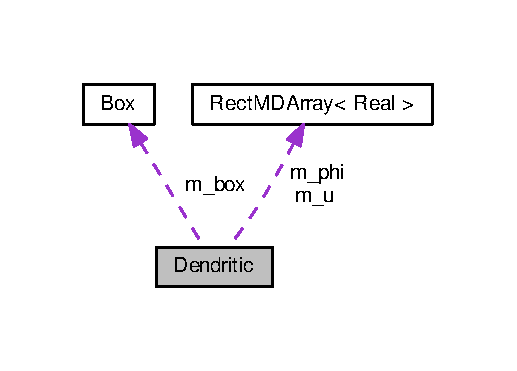
\includegraphics[width=248pt]{classDendritic__coll__graph}
\end{center}
\end{figure}
\subsection*{Public Member Functions}
\begin{DoxyCompactItemize}
\item 
\hypertarget{classDendritic_afefc8047c94056afaa56617c24518a1e}{}{\bfseries Dendritic} (\hyperlink{classBox}{Box} \&a\+\_\+box, \hyperlink{classRectMDArray}{Rect\+M\+D\+Array}$<$ Real $>$ \&phi\+\_\+int, \hyperlink{classRectMDArray}{Rect\+M\+D\+Array}$<$ Real $>$ \&u\+\_\+int)\label{classDendritic_afefc8047c94056afaa56617c24518a1e}

\item 
\hypertarget{classDendritic_a152a728fd7bac656f0d322d0e844dec8}{}void {\bfseries increment} (const \hyperlink{classDendriticShift}{Dendritic\+Shift} \&a\+\_\+shift)\label{classDendritic_a152a728fd7bac656f0d322d0e844dec8}

\end{DoxyCompactItemize}
\subsection*{Public Attributes}
\begin{DoxyCompactItemize}
\item 
\hypertarget{classDendritic_a4cde2313fd108d64c94eb58829c1b8d4}{}bool {\bfseries m\+\_\+is\+Defined}\label{classDendritic_a4cde2313fd108d64c94eb58829c1b8d4}

\item 
\hypertarget{classDendritic_a027e1104026bbde26dc050c67dbc6808}{}\hyperlink{classBox}{Box} {\bfseries m\+\_\+box}\label{classDendritic_a027e1104026bbde26dc050c67dbc6808}

\item 
\hypertarget{classDendritic_a5d2ebb6ba207172b5c00fd3d43173fbd}{}\hyperlink{classRectMDArray}{Rect\+M\+D\+Array}$<$ Real $>$ {\bfseries m\+\_\+phi}\label{classDendritic_a5d2ebb6ba207172b5c00fd3d43173fbd}

\item 
\hypertarget{classDendritic_a2bdf3ee8b87990e6d67bd341905235f3}{}\hyperlink{classRectMDArray}{Rect\+M\+D\+Array}$<$ Real $>$ {\bfseries m\+\_\+u}\label{classDendritic_a2bdf3ee8b87990e6d67bd341905235f3}

\end{DoxyCompactItemize}


The documentation for this class was generated from the following files\+:\begin{DoxyCompactItemize}
\item 
/home/xingjie/\+Documents/grad\+School/courses/software\+Eng\+For\+Sci\+Comp/final\+Project/github\+Repo/\+C\+S294-\/73/code/src/\+Dendritic/Dendritic.\+H\item 
/home/xingjie/\+Documents/grad\+School/courses/software\+Eng\+For\+Sci\+Comp/final\+Project/github\+Repo/\+C\+S294-\/73/code/src/\+Dendritic/Dendritic.\+cpp\end{DoxyCompactItemize}

\hypertarget{classDendriticGrowth}{}\section{Dendritic\+Growth Class Reference}
\label{classDendriticGrowth}\index{Dendritic\+Growth@{Dendritic\+Growth}}
\subsection*{Public Member Functions}
\begin{DoxyCompactItemize}
\item 
\hypertarget{classDendriticGrowth_a30dda5137def030d930785b7a39e5cfd}{}bool {\bfseries is\+Defined} ()\label{classDendriticGrowth_a30dda5137def030d930785b7a39e5cfd}

\item 
\hypertarget{classDendriticGrowth_a29ccda56e5679491032a2136acb515e6}{}void {\bfseries operator()} (\hyperlink{classDendriticShift}{Dendritic\+Shift} \&a\+\_\+k, const Real \&a\+\_\+time, const Real \&dt, \hyperlink{classDendritic}{Dendritic} \&a\+\_\+state)\label{classDendriticGrowth_a29ccda56e5679491032a2136acb515e6}

\end{DoxyCompactItemize}
\subsection*{Public Attributes}
\begin{DoxyCompactItemize}
\item 
\hypertarget{classDendriticGrowth_aaf51aef6cfbe16561b8dd15aa8fe3d3f}{}Real {\bfseries m\+\_\+h}\label{classDendriticGrowth_aaf51aef6cfbe16561b8dd15aa8fe3d3f}

\item 
\hypertarget{classDendriticGrowth_af951d2b367dc6116ca8ecdfdd21dc3d5}{}Real {\bfseries m\+\_\+\+D}\label{classDendriticGrowth_af951d2b367dc6116ca8ecdfdd21dc3d5}

\item 
\hypertarget{classDendriticGrowth_af0870181a7d16647abac756a98b95af8}{}Real {\bfseries m\+\_\+tau}\label{classDendriticGrowth_af0870181a7d16647abac756a98b95af8}

\item 
\hypertarget{classDendriticGrowth_ae6f3f44b8852fed02d58e107ee55d4c8}{}Real {\bfseries m\+\_\+beta}\label{classDendriticGrowth_ae6f3f44b8852fed02d58e107ee55d4c8}

\item 
\hypertarget{classDendriticGrowth_ad2712d9eba7cc0a4320bcec2f61e58db}{}Real {\bfseries m\+\_\+eta}\label{classDendriticGrowth_ad2712d9eba7cc0a4320bcec2f61e58db}

\item 
\hypertarget{classDendriticGrowth_a28930e8b2f322f9b2347f78d5cef4f9d}{}Real {\bfseries m\+\_\+um}\label{classDendriticGrowth_a28930e8b2f322f9b2347f78d5cef4f9d}

\item 
\hypertarget{classDendriticGrowth_a2b9d113fa4a03df3086da8816176b645}{}Real {\bfseries m\+\_\+\+W0}\label{classDendriticGrowth_a2b9d113fa4a03df3086da8816176b645}

\item 
\hypertarget{classDendriticGrowth_afb851c0005f573d9b8bbf87416baae26}{}Real {\bfseries m\+\_\+mu}\label{classDendriticGrowth_afb851c0005f573d9b8bbf87416baae26}

\item 
\hypertarget{classDendriticGrowth_a544b2e1320949f4d06a2edd06a8cab6b}{}Real {\bfseries m\+\_\+a0}\label{classDendriticGrowth_a544b2e1320949f4d06a2edd06a8cab6b}

\item 
\hypertarget{classDendriticGrowth_a52bbb6db7885f3472e4cef7b8ec9513d}{}Real {\bfseries m\+\_\+theta0}\label{classDendriticGrowth_a52bbb6db7885f3472e4cef7b8ec9513d}

\end{DoxyCompactItemize}


The documentation for this class was generated from the following files\+:\begin{DoxyCompactItemize}
\item 
/home/xingjie/\+Documents/grad\+School/courses/software\+Eng\+For\+Sci\+Comp/final\+Project/github\+Repo/\+C\+S294-\/73/code/src/\+Dendritic/Dendritic\+Growth.\+H\item 
/home/xingjie/\+Documents/grad\+School/courses/software\+Eng\+For\+Sci\+Comp/final\+Project/github\+Repo/\+C\+S294-\/73/code/src/\+Dendritic/Dendritic\+Growth.\+cpp\end{DoxyCompactItemize}

\hypertarget{classDendriticShift}{}\section{Dendritic\+Shift Class Reference}
\label{classDendriticShift}\index{Dendritic\+Shift@{Dendritic\+Shift}}


Collaboration diagram for Dendritic\+Shift\+:
\nopagebreak
\begin{figure}[H]
\begin{center}
\leavevmode
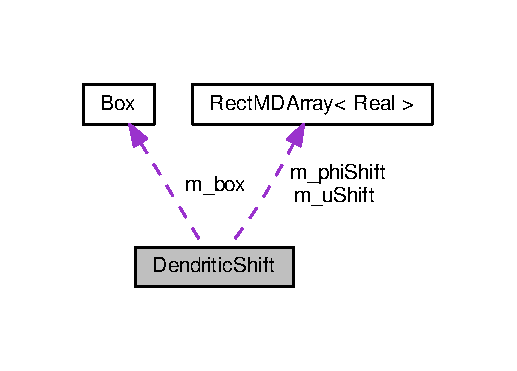
\includegraphics[width=248pt]{classDendriticShift__coll__graph}
\end{center}
\end{figure}
\subsection*{Public Member Functions}
\begin{DoxyCompactItemize}
\item 
\hypertarget{classDendriticShift_adee89364f91a569e90602b6c40ecd9f0}{}void {\bfseries init} (const \hyperlink{classDendritic}{Dendritic} \&a\+\_\+dendritic)\label{classDendriticShift_adee89364f91a569e90602b6c40ecd9f0}

\item 
\hypertarget{classDendriticShift_a4eeae0e689cf4fa7c5cdacfd2420d260}{}void {\bfseries increment} (double a\+\_\+scale, const \hyperlink{classDendriticShift}{Dendritic\+Shift} \&a\+\_\+rhs)\label{classDendriticShift_a4eeae0e689cf4fa7c5cdacfd2420d260}

\item 
\hypertarget{classDendriticShift_ab97d5c358ddafa3ff7fb6d13cdc3521a}{}void {\bfseries operator$\ast$=} (double a\+\_\+scale)\label{classDendriticShift_ab97d5c358ddafa3ff7fb6d13cdc3521a}

\item 
\hypertarget{classDendriticShift_aa195e2e73dffff676d52bcf39c367cdb}{}void {\bfseries set\+To\+Zero} ()\label{classDendriticShift_aa195e2e73dffff676d52bcf39c367cdb}

\end{DoxyCompactItemize}
\subsection*{Public Attributes}
\begin{DoxyCompactItemize}
\item 
\hypertarget{classDendriticShift_a08c611e07c85d23f1822f03775a217f5}{}\hyperlink{classBox}{Box} {\bfseries m\+\_\+box}\label{classDendriticShift_a08c611e07c85d23f1822f03775a217f5}

\item 
\hypertarget{classDendriticShift_acad8e4fc5c384d7bce09f9c998d4643e}{}\hyperlink{classRectMDArray}{Rect\+M\+D\+Array}$<$ Real $>$ {\bfseries m\+\_\+phi\+Shift}\label{classDendriticShift_acad8e4fc5c384d7bce09f9c998d4643e}

\item 
\hypertarget{classDendriticShift_a710068a8ab51f0830cc6f7f304a97509}{}\hyperlink{classRectMDArray}{Rect\+M\+D\+Array}$<$ Real $>$ {\bfseries m\+\_\+u\+Shift}\label{classDendriticShift_a710068a8ab51f0830cc6f7f304a97509}

\end{DoxyCompactItemize}


The documentation for this class was generated from the following files\+:\begin{DoxyCompactItemize}
\item 
/home/xingjie/\+Documents/grad\+School/courses/software\+Eng\+For\+Sci\+Comp/final\+Project/github\+Repo/\+C\+S294-\/73/code/src/\+Dendritic/Dendritic.\+H\item 
/home/xingjie/\+Documents/grad\+School/courses/software\+Eng\+For\+Sci\+Comp/final\+Project/github\+Repo/\+C\+S294-\/73/code/src/\+Dendritic/Dendritic.\+cpp\end{DoxyCompactItemize}

\hypertarget{structelem}{}\section{elem Struct Reference}
\label{structelem}\index{elem@{elem}}


Collaboration diagram for elem\+:
\nopagebreak
\begin{figure}[H]
\begin{center}
\leavevmode
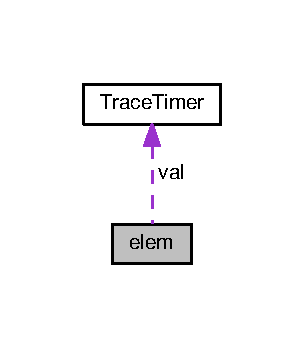
\includegraphics[width=146pt]{structelem__coll__graph}
\end{center}
\end{figure}
\subsection*{Public Member Functions}
\begin{DoxyCompactItemize}
\item 
\hypertarget{structelem_a1b3c3f35e36509cd5c5d4b58d2cd2c4b}{}{\bfseries elem} (const \hyperlink{classTraceTimer}{Trace\+Timer} $\ast$p, unsigned long long int t)\label{structelem_a1b3c3f35e36509cd5c5d4b58d2cd2c4b}

\item 
\hypertarget{structelem_a63a278276a0c0ba917d363366dfd57b4}{}bool {\bfseries operator$<$} (const \hyperlink{structelem}{elem} \&rhs) const \label{structelem_a63a278276a0c0ba917d363366dfd57b4}

\end{DoxyCompactItemize}
\subsection*{Static Public Member Functions}
\begin{DoxyCompactItemize}
\item 
\hypertarget{structelem_a89030e25e760d130062432961126f9c9}{}static void {\bfseries build\+List} (std\+::list$<$ \hyperlink{structelem}{elem} $>$ \&tlist, const \hyperlink{classTraceTimer}{Trace\+Timer} \&timer)\label{structelem_a89030e25e760d130062432961126f9c9}

\end{DoxyCompactItemize}
\subsection*{Public Attributes}
\begin{DoxyCompactItemize}
\item 
\hypertarget{structelem_a70c81057f0b23f069da106d48887d445}{}const \hyperlink{classTraceTimer}{Trace\+Timer} $\ast$ {\bfseries val}\label{structelem_a70c81057f0b23f069da106d48887d445}

\item 
\hypertarget{structelem_abcb627f67401148616c650951b93b50e}{}unsigned long long int {\bfseries time}\label{structelem_abcb627f67401148616c650951b93b50e}

\end{DoxyCompactItemize}


The documentation for this struct was generated from the following file\+:\begin{DoxyCompactItemize}
\item 
/home/xingjie/\+Documents/grad\+School/courses/software\+Eng\+For\+Sci\+Comp/final\+Project/github\+Repo/\+C\+S294-\/73/code/src/\+Timer/C\+H\+\_\+\+Timer.\+cpp\end{DoxyCompactItemize}

\hypertarget{classPoint}{}\section{Point Class Reference}
\label{classPoint}\index{Point@{Point}}
\subsection*{Public Member Functions}
\begin{DoxyCompactItemize}
\item 
\hypertarget{classPoint_ad92f2337b839a94ce97dcdb439b4325a}{}\hyperlink{classPoint_ad92f2337b839a94ce97dcdb439b4325a}{Point} ()\label{classPoint_ad92f2337b839a94ce97dcdb439b4325a}

\begin{DoxyCompactList}\small\item\em Default Constructor. \end{DoxyCompactList}\item 
\hypertarget{classPoint_ad2979175ac77062182ecfae283c8b97f}{}\hyperlink{classPoint_ad2979175ac77062182ecfae283c8b97f}{Point} (const int a\+\_\+tuple\mbox{[}D\+I\+M\mbox{]})\label{classPoint_ad2979175ac77062182ecfae283c8b97f}

\begin{DoxyCompactList}\small\item\em Constructor. \end{DoxyCompactList}\item 
\hypertarget{classPoint_ad3049b9597a2dc93be3fc304bbf3cdbb}{}\hyperlink{classPoint_ad3049b9597a2dc93be3fc304bbf3cdbb}{Point} (const \hyperlink{classPoint}{Point} \&a\+\_\+pt)\label{classPoint_ad3049b9597a2dc93be3fc304bbf3cdbb}

\begin{DoxyCompactList}\small\item\em Copy constructor. \end{DoxyCompactList}\item 
\hypertarget{classPoint_a52e66dbfdd8eb6929caf289af61d182a}{}\hyperlink{classPoint}{Point} \hyperlink{classPoint_a52e66dbfdd8eb6929caf289af61d182a}{operator+} (const \hyperlink{classPoint}{Point} \&a\+\_\+rhs\+Point) const \label{classPoint_a52e66dbfdd8eb6929caf289af61d182a}

\begin{DoxyCompactList}\small\item\em Adds two points. \end{DoxyCompactList}\item 
\hypertarget{classPoint_ad93f0f1d1a4247ade4e08f2e546f6fcf}{}\hyperlink{classPoint}{Point} \hyperlink{classPoint_ad93f0f1d1a4247ade4e08f2e546f6fcf}{operator-\/} (const \hyperlink{classPoint}{Point} \&a\+\_\+rhs\+Point) const \label{classPoint_ad93f0f1d1a4247ade4e08f2e546f6fcf}

\begin{DoxyCompactList}\small\item\em Subtracts two points. \end{DoxyCompactList}\item 
\hypertarget{classPoint_a59eae349066f8366ccf97c129c33d276}{}\hyperlink{classPoint}{Point} \hyperlink{classPoint_a59eae349066f8366ccf97c129c33d276}{operator/} (int a\+\_\+nref) const \label{classPoint_a59eae349066f8366ccf97c129c33d276}

\begin{DoxyCompactList}\small\item\em division by an integer -\/ rounds down. \end{DoxyCompactList}\item 
\hypertarget{classPoint_ad7644e8ecf6313d23605562788dfb995}{}\hyperlink{classPoint}{Point} \hyperlink{classPoint_ad7644e8ecf6313d23605562788dfb995}{operator/} (const \hyperlink{classPoint}{Point} \&a\+\_\+pt) const \label{classPoint_ad7644e8ecf6313d23605562788dfb995}

\begin{DoxyCompactList}\small\item\em Componentwise division by a \hyperlink{classPoint}{Point} -\/ rounds down. \end{DoxyCompactList}\item 
\hypertarget{classPoint_a4152c209ab56ba52931febfd97f87c3c}{}\hyperlink{classPoint}{Point} \hyperlink{classPoint_a4152c209ab56ba52931febfd97f87c3c}{operator$\ast$} (int a\+\_\+nref) const \label{classPoint_a4152c209ab56ba52931febfd97f87c3c}

\begin{DoxyCompactList}\small\item\em multiplication by an integer. \end{DoxyCompactList}\item 
\hypertarget{classPoint_acc7e19bbf8de57b34764727b671b839e}{}\hyperlink{classPoint}{Point} \hyperlink{classPoint_acc7e19bbf8de57b34764727b671b839e}{operator$\ast$} (const \hyperlink{classPoint}{Point} \&a\+\_\+pt) const \label{classPoint_acc7e19bbf8de57b34764727b671b839e}

\begin{DoxyCompactList}\small\item\em Componentwise multiplication by a \hyperlink{classPoint}{Point}. \end{DoxyCompactList}\item 
\hypertarget{classPoint_ab7db9ac762d6637efcce56afc7750f1f}{}void \hyperlink{classPoint_ab7db9ac762d6637efcce56afc7750f1f}{operator$\ast$=} (const \hyperlink{classPoint}{Point} \&a\+\_\+pt)\label{classPoint_ab7db9ac762d6637efcce56afc7750f1f}

\begin{DoxyCompactList}\small\item\em Update in place arithmetic operations. \end{DoxyCompactList}\item 
\hypertarget{classPoint_a587465b64c61c24c7bcb9abf0dfda114}{}void {\bfseries operator+=} (const \hyperlink{classPoint}{Point} \&a\+\_\+pt)\label{classPoint_a587465b64c61c24c7bcb9abf0dfda114}

\item 
\hypertarget{classPoint_a5c41a95bd50b076bdca75d920f73554f}{}void {\bfseries operator-\/=} (const \hyperlink{classPoint}{Point} \&a\+\_\+pt)\label{classPoint_a5c41a95bd50b076bdca75d920f73554f}

\item 
\hypertarget{classPoint_a61672dab6c26441eac5aca9928cdfc1f}{}void {\bfseries operator/=} (const \hyperlink{classPoint}{Point} \&a\+\_\+pt)\label{classPoint_a61672dab6c26441eac5aca9928cdfc1f}

\item 
\hypertarget{classPoint_a79d9895cf934366e864a69a483e5b8ad}{}void \hyperlink{classPoint_a79d9895cf934366e864a69a483e5b8ad}{operator$\ast$=} (int a\+\_\+n)\label{classPoint_a79d9895cf934366e864a69a483e5b8ad}

\begin{DoxyCompactList}\small\item\em Update in place aritmetic operations. Adds integer to every component. \end{DoxyCompactList}\item 
\hypertarget{classPoint_ae6e49461a0bc525c0f55bd5ce42db45b}{}void {\bfseries operator+=} (int a\+\_\+n)\label{classPoint_ae6e49461a0bc525c0f55bd5ce42db45b}

\item 
\hypertarget{classPoint_a880f2ce648e6011177058678f6b2021b}{}void {\bfseries operator-\/=} (int a\+\_\+n)\label{classPoint_a880f2ce648e6011177058678f6b2021b}

\item 
\hypertarget{classPoint_a62ab14874fced136ff69ed4cf6d34c90}{}void {\bfseries operator/=} (int a\+\_\+n)\label{classPoint_a62ab14874fced136ff69ed4cf6d34c90}

\item 
\hypertarget{classPoint_a40ee8f921d2641d6380188419e4885b3}{}bool \hyperlink{classPoint_a40ee8f921d2641d6380188419e4885b3}{operator==} (const \hyperlink{classPoint}{Point} \&a\+\_\+pt) const \label{classPoint_a40ee8f921d2641d6380188419e4885b3}

\begin{DoxyCompactList}\small\item\em are two points equal. \end{DoxyCompactList}\item 
\hypertarget{classPoint_a88c0a9d6ac6824e141dce78941996edf}{}const int \& \hyperlink{classPoint_a88c0a9d6ac6824e141dce78941996edf}{operator\mbox{[}$\,$\mbox{]}} (const int \&a\+\_\+index) const \label{classPoint_a88c0a9d6ac6824e141dce78941996edf}

\begin{DoxyCompactList}\small\item\em Get a component of a point. \end{DoxyCompactList}\end{DoxyCompactItemize}


The documentation for this class was generated from the following files\+:\begin{DoxyCompactItemize}
\item 
/home/xingjie/\+Documents/grad\+School/courses/software\+Eng\+For\+Sci\+Comp/final\+Project/github\+Repo/\+C\+S294-\/73/code/src/\+Rect\+Array/Point.\+H\item 
/home/xingjie/\+Documents/grad\+School/courses/software\+Eng\+For\+Sci\+Comp/final\+Project/github\+Repo/\+C\+S294-\/73/code/src/\+Rect\+Array/Point\+Implem.\+H\end{DoxyCompactItemize}

\hypertarget{classRectMDArray}{}\section{Rect\+M\+D\+Array$<$ T $>$ Class Template Reference}
\label{classRectMDArray}\index{Rect\+M\+D\+Array$<$ T $>$@{Rect\+M\+D\+Array$<$ T $>$}}
\subsection*{Public Member Functions}
\begin{DoxyCompactItemize}
\item 
\hypertarget{classRectMDArray_ac00866b851e65694dd67da2bcb66589b}{}\hyperlink{classRectMDArray_ac00866b851e65694dd67da2bcb66589b}{Rect\+M\+D\+Array} ()\label{classRectMDArray_ac00866b851e65694dd67da2bcb66589b}

\begin{DoxyCompactList}\small\item\em Default constructor. \end{DoxyCompactList}\item 
\hypertarget{classRectMDArray_a3ebeb8a94543970a6e4c04e97bb09407}{}\hyperlink{classRectMDArray_a3ebeb8a94543970a6e4c04e97bb09407}{Rect\+M\+D\+Array} (const \hyperlink{classBox}{Box} \&a\+\_\+box)\label{classRectMDArray_a3ebeb8a94543970a6e4c04e97bb09407}

\begin{DoxyCompactList}\small\item\em Constructs an \hyperlink{classRectMDArray}{Rect\+M\+D\+Array} over the \hyperlink{classBox}{Box} a\+\_\+box;. \end{DoxyCompactList}\item 
\hypertarget{classRectMDArray_a4eac73fde8106984c7970fab82b2c146}{}void \hyperlink{classRectMDArray_a4eac73fde8106984c7970fab82b2c146}{define} (const \hyperlink{classBox}{Box} \&a\+\_\+box)\label{classRectMDArray_a4eac73fde8106984c7970fab82b2c146}

\begin{DoxyCompactList}\small\item\em Defines a default-\/constructed \hyperlink{classRectMDArray}{Rect\+M\+D\+Array}. \end{DoxyCompactList}\item 
\hypertarget{classRectMDArray_ae151647324ccd43e30a893a1edb03e83}{}\hyperlink{classRectMDArray_ae151647324ccd43e30a893a1edb03e83}{Rect\+M\+D\+Array} (const \hyperlink{classRectMDArray}{Rect\+M\+D\+Array}$<$ T $>$ \&a\+\_\+src\+Array)\label{classRectMDArray_ae151647324ccd43e30a893a1edb03e83}

\begin{DoxyCompactList}\small\item\em Copy constructor. \end{DoxyCompactList}\item 
\hypertarget{classRectMDArray_a098d6879255ce1fe43fe03c1f8460a6b}{}\hyperlink{classRectMDArray_a098d6879255ce1fe43fe03c1f8460a6b}{$\sim$\+Rect\+M\+D\+Array} ()\label{classRectMDArray_a098d6879255ce1fe43fe03c1f8460a6b}

\begin{DoxyCompactList}\small\item\em Destructor. \end{DoxyCompactList}\item 
\hypertarget{classRectMDArray_a3e18c24dc02c6354f201a8261493d248}{}void \hyperlink{classRectMDArray_a3e18c24dc02c6354f201a8261493d248}{set\+Val} (const T \&a\+\_\+val)\label{classRectMDArray_a3e18c24dc02c6354f201a8261493d248}

\begin{DoxyCompactList}\small\item\em Setting an \hyperlink{classRectMDArray}{Rect\+M\+D\+Array} to a constant value. \end{DoxyCompactList}\item 
\hypertarget{classRectMDArray_a5ab74c7822c98485daf7c974e5149c91}{}\hyperlink{classRectMDArray}{Rect\+M\+D\+Array} \& \hyperlink{classRectMDArray_a5ab74c7822c98485daf7c974e5149c91}{operator=} (const \hyperlink{classRectMDArray}{Rect\+M\+D\+Array}$<$ T $>$ \&a\+\_\+src\+Array)\label{classRectMDArray_a5ab74c7822c98485daf7c974e5149c91}

\begin{DoxyCompactList}\small\item\em Assignment operator. \end{DoxyCompactList}\item 
\hypertarget{classRectMDArray_a25ab8a23bb0791906bd9f69adffaf257}{}\hyperlink{classBox}{Box} \hyperlink{classRectMDArray_a25ab8a23bb0791906bd9f69adffaf257}{get\+Box} () const \label{classRectMDArray_a25ab8a23bb0791906bd9f69adffaf257}

\begin{DoxyCompactList}\small\item\em Gets box over which array is defined. \end{DoxyCompactList}\item 
\hypertarget{classRectMDArray_acb19cbfddee6a5a1610e49bbb6deed9e}{}T \& \hyperlink{classRectMDArray_acb19cbfddee6a5a1610e49bbb6deed9e}{operator\mbox{[}$\,$\mbox{]}} (const \hyperlink{classPoint}{Point} \&a\+\_\+iv) const \label{classRectMDArray_acb19cbfddee6a5a1610e49bbb6deed9e}

\begin{DoxyCompactList}\small\item\em Indexing operator. \end{DoxyCompactList}\item 
\hypertarget{classRectMDArray_aade82e1d2165ca7382f04a30f898e749}{}T $\ast$ \hyperlink{classRectMDArray_aade82e1d2165ca7382f04a30f898e749}{get\+Pointer} () const \label{classRectMDArray_aade82e1d2165ca7382f04a30f898e749}

\begin{DoxyCompactList}\small\item\em get raw pointer. \end{DoxyCompactList}\item 
\hypertarget{classRectMDArray_a65d54efccaa796e05375cb0f9a477a36}{}T \& \hyperlink{classRectMDArray_a65d54efccaa796e05375cb0f9a477a36}{operator\mbox{[}$\,$\mbox{]}} (int a\+\_\+index) const \label{classRectMDArray_a65d54efccaa796e05375cb0f9a477a36}

\begin{DoxyCompactList}\small\item\em Index with integer. \end{DoxyCompactList}\item 
\hypertarget{classRectMDArray_a519144a95692a9e6aabadbd80e8da4b9}{}T \& {\bfseries val} (int a\+\_\+index)\label{classRectMDArray_a519144a95692a9e6aabadbd80e8da4b9}

\end{DoxyCompactItemize}


The documentation for this class was generated from the following files\+:\begin{DoxyCompactItemize}
\item 
/home/xingjie/\+Documents/grad\+School/courses/software\+Eng\+For\+Sci\+Comp/final\+Project/github\+Repo/\+C\+S294-\/73/code/src/\+Rect\+Array/Rect\+M\+D\+Array.\+H\item 
/home/xingjie/\+Documents/grad\+School/courses/software\+Eng\+For\+Sci\+Comp/final\+Project/github\+Repo/\+C\+S294-\/73/code/src/\+Rect\+Array/Rect\+M\+D\+Array\+Implem.\+H\end{DoxyCompactItemize}

\hypertarget{classRectMDOperators}{}\section{Rect\+M\+D\+Operators Class Reference}
\label{classRectMDOperators}\index{Rect\+M\+D\+Operators@{Rect\+M\+D\+Operators}}


This class is a set of operators that act on \hyperlink{classRectMDArray}{Rect\+M\+D\+Array} and a given point. All of the operators are dimension independent.  




{\ttfamily \#include $<$Rect\+M\+D\+Operators.\+H$>$}

\subsection*{Public Member Functions}
\begin{DoxyCompactItemize}
\item 
\hypertarget{classRectMDOperators_a64e546d7304f8a28782683a7788b7023}{}Real {\bfseries get\+Laplacian} (const \hyperlink{classRectMDArray}{Rect\+M\+D\+Array}$<$ Real $>$ \&a\+\_\+field, const \hyperlink{classPoint}{Point} \&a\+\_\+p, Real a\+\_\+h)\label{classRectMDOperators_a64e546d7304f8a28782683a7788b7023}

\item 
\hypertarget{classRectMDOperators_a52d79cf50e2eba08f70725de6b8d06dd}{}array$<$ Real, D\+I\+M $>$ {\bfseries get\+Gradient} (const \hyperlink{classRectMDArray}{Rect\+M\+D\+Array}$<$ Real $>$ \&a\+\_\+field, const \hyperlink{classPoint}{Point} \&a\+\_\+p, Real a\+\_\+h)\label{classRectMDOperators_a52d79cf50e2eba08f70725de6b8d06dd}

\item 
\hypertarget{classRectMDOperators_a98c69a17cb3e734bf0b87b88f3a58a44}{}Real {\bfseries get\+Divergence} (const \hyperlink{classRectMDArray}{Rect\+M\+D\+Array}$<$ array$<$ Real, D\+I\+M $>$ $>$ \&a\+\_\+vec\+Field, const \hyperlink{classPoint}{Point} \&a\+\_\+p, Real a\+\_\+h)\label{classRectMDOperators_a98c69a17cb3e734bf0b87b88f3a58a44}

\item 
\hypertarget{classRectMDOperators_aa2ed5097ef35e88f23d69113da58f101}{}void {\bfseries get\+Laplacian\+Field} (const \hyperlink{classRectMDArray}{Rect\+M\+D\+Array}$<$ Real $>$ \&a\+\_\+field, \hyperlink{classRectMDArray}{Rect\+M\+D\+Array}$<$ Real $>$ \&a\+\_\+lap\+Field, Real a\+\_\+h)\label{classRectMDOperators_aa2ed5097ef35e88f23d69113da58f101}

\item 
\hypertarget{classRectMDOperators_ae9fc7ba894b8235f33b8f9ca2d36cf16}{}void {\bfseries get\+Gradient\+Field} (const \hyperlink{classRectMDArray}{Rect\+M\+D\+Array}$<$ Real $>$ \&a\+\_\+field, \hyperlink{classRectMDArray}{Rect\+M\+D\+Array}$<$ array$<$ Real, D\+I\+M $>$ $>$ \&a\+\_\+grad\+Field, Real a\+\_\+h)\label{classRectMDOperators_ae9fc7ba894b8235f33b8f9ca2d36cf16}

\item 
\hypertarget{classRectMDOperators_aecd7c2ab2082c8e0d20fb519c4151254}{}void {\bfseries get\+Divergence\+Field} (const \hyperlink{classRectMDArray}{Rect\+M\+D\+Array}$<$ array$<$ Real, D\+I\+M $>$ $>$ \&a\+\_\+vec\+Field, \hyperlink{classRectMDArray}{Rect\+M\+D\+Array}$<$ Real $>$ \&a\+\_\+div\+Field, Real a\+\_\+h)\label{classRectMDOperators_aecd7c2ab2082c8e0d20fb519c4151254}

\end{DoxyCompactItemize}


\subsection{Detailed Description}
This class is a set of operators that act on \hyperlink{classRectMDArray}{Rect\+M\+D\+Array} and a given point. All of the operators are dimension independent. 

The documentation for this class was generated from the following files\+:\begin{DoxyCompactItemize}
\item 
/home/xingjie/\+Documents/grad\+School/courses/software\+Eng\+For\+Sci\+Comp/final\+Project/github\+Repo/\+C\+S294-\/73/code/src/\+Dendritic/Rect\+M\+D\+Operators.\+H\item 
/home/xingjie/\+Documents/grad\+School/courses/software\+Eng\+For\+Sci\+Comp/final\+Project/github\+Repo/\+C\+S294-\/73/code/src/\+Dendritic/Rect\+M\+D\+Operators.\+cpp\end{DoxyCompactItemize}

\hypertarget{classRK4}{}\section{R\+K4$<$ X, F, d\+X $>$ Class Template Reference}
\label{classRK4}\index{R\+K4$<$ X, F, d\+X $>$@{R\+K4$<$ X, F, d\+X $>$}}


generic explicit \hyperlink{classRK4}{R\+K4} algorithm  




{\ttfamily \#include $<$R\+K4.\+H$>$}

\subsection*{Public Member Functions}
\begin{DoxyCompactItemize}
\item 
\hypertarget{classRK4_af0486f7e162b0a935b390bb7fc1a9f02}{}void {\bfseries advance} (double a\+\_\+time, double a\+\_\+dt, X \&a\+\_\+state)\label{classRK4_af0486f7e162b0a935b390bb7fc1a9f02}

\end{DoxyCompactItemize}
\subsection*{Protected Attributes}
\begin{DoxyCompactItemize}
\item 
\hypertarget{classRK4_a92f523886ca69913832d9efae83579ac}{}d\+X {\bfseries m\+\_\+k}\label{classRK4_a92f523886ca69913832d9efae83579ac}

\item 
\hypertarget{classRK4_ab79f59c90025ff0f04fa3391fd0a6e4b}{}d\+X {\bfseries m\+\_\+delta}\label{classRK4_ab79f59c90025ff0f04fa3391fd0a6e4b}

\item 
\hypertarget{classRK4_a8708d55158344f113a14ec23fec25a91}{}F {\bfseries m\+\_\+f}\label{classRK4_a8708d55158344f113a14ec23fec25a91}

\end{DoxyCompactItemize}


\subsection{Detailed Description}
\subsubsection*{template$<$class X, class F, class d\+X$>$class R\+K4$<$ X, F, d\+X $>$}

generic explicit \hyperlink{classRK4}{R\+K4} algorithm 

class X is the type of your state data. class F provides an evaluation of the X\textquotesingle{} for a specified state of X and the time. If your X\textquotesingle{} is determined entirely from the current state values then F can ignore. F implements the function\+: void operator(\+X\& k, double a\+\_\+time, double a\+\_\+dt, const X\& a\+\_\+state, const X\& a\+\_\+shift);

F interprets the real state as a\+\_\+state+a\+\_\+shift

Note that F includes the customary factor of d\+T in the \hyperlink{classRK4}{R\+K4} algorithm. (i.\+e. this algorithm assumes k\+\_\+i = F(...) N\+O\+T k\+\_\+i = dt$\ast$\+F(...) 

The documentation for this class was generated from the following file\+:\begin{DoxyCompactItemize}
\item 
/home/xingjie/\+Documents/grad\+School/courses/software\+Eng\+For\+Sci\+Comp/final\+Project/github\+Repo/\+C\+S294-\/73/code/src/\+Dendritic/R\+K4.\+H\end{DoxyCompactItemize}

\hypertarget{classTraceTimer}{}\section{Trace\+Timer Class Reference}
\label{classTraceTimer}\index{Trace\+Timer@{Trace\+Timer}}


{\ttfamily \#include $<$C\+H\+\_\+\+Timer.\+H$>$}

\subsection*{Public Member Functions}
\begin{DoxyCompactItemize}
\item 
\hypertarget{classTraceTimer_a03205e8ad8c9ce4564d686707f82fe84}{}void {\bfseries start} (char $\ast$mutex)\label{classTraceTimer_a03205e8ad8c9ce4564d686707f82fe84}

\item 
\hypertarget{classTraceTimer_a690e043d786547decec8c483cf662ca1}{}unsigned long long int {\bfseries stop} (char $\ast$mutex)\label{classTraceTimer_a690e043d786547decec8c483cf662ca1}

\item 
\hypertarget{classTraceTimer_adf7648634d5812e6d9d5de15f00e8314}{}void {\bfseries leaf\+Start} ()\label{classTraceTimer_adf7648634d5812e6d9d5de15f00e8314}

\item 
\hypertarget{classTraceTimer_a79a39ed75671663311d05fcfbb9c4ad7}{}void {\bfseries leaf\+Stop} ()\label{classTraceTimer_a79a39ed75671663311d05fcfbb9c4ad7}

\item 
\hypertarget{classTraceTimer_a3444db7e0d172bc7af48b06a252c7280}{}unsigned long long int {\bfseries time} () const \label{classTraceTimer_a3444db7e0d172bc7af48b06a252c7280}

\item 
\hypertarget{classTraceTimer_a679c13c59b83fa01f49c5d5b06509718}{}int {\bfseries rank} () const \label{classTraceTimer_a679c13c59b83fa01f49c5d5b06509718}

\item 
\hypertarget{classTraceTimer_a9bb6e59b5595ef2304e1054c7fc5b38c}{}long long int {\bfseries count} () const \label{classTraceTimer_a9bb6e59b5595ef2304e1054c7fc5b38c}

\item 
\hypertarget{classTraceTimer_a368f32b604ecd500afb084851e8c51ce}{}void {\bfseries prune} ()\label{classTraceTimer_a368f32b604ecd500afb084851e8c51ce}

\item 
\hypertarget{classTraceTimer_ae9de90ae7a635f77a2eca9911853888d}{}bool {\bfseries is\+Pruned} () const \label{classTraceTimer_ae9de90ae7a635f77a2eca9911853888d}

\item 
\hypertarget{classTraceTimer_afda09014b2657611d6918bcc9b8b6943}{}const std\+::vector$<$ \hyperlink{classTraceTimer}{Trace\+Timer} $\ast$ $>$ \& {\bfseries children} () const \label{classTraceTimer_afda09014b2657611d6918bcc9b8b6943}

\end{DoxyCompactItemize}
\subsection*{Static Public Member Functions}
\begin{DoxyCompactItemize}
\item 
\hypertarget{classTraceTimer_a099a00979dce21aa8152189caa9e3664}{}static void {\bfseries report} (bool a\+\_\+close\+After=false)\label{classTraceTimer_a099a00979dce21aa8152189caa9e3664}

\item 
\hypertarget{classTraceTimer_a9c51438e2ce920545955f6b03d1959aa}{}static void {\bfseries reset} ()\label{classTraceTimer_a9c51438e2ce920545955f6b03d1959aa}

\item 
\hypertarget{classTraceTimer_ad2418f864f19ff1af50a7dd86d1ac572}{}static int {\bfseries initializer} ()\label{classTraceTimer_ad2418f864f19ff1af50a7dd86d1ac572}

\item 
\hypertarget{classTraceTimer_a2f3e79338d3f21acc37bcf9a12cc67ae}{}static \hyperlink{classTraceTimer}{Trace\+Timer} $\ast$ {\bfseries get\+Timer} (const char $\ast$name)\label{classTraceTimer_a2f3e79338d3f21acc37bcf9a12cc67ae}

\item 
\hypertarget{classTraceTimer_a5195aa7537a7db853ce2ec8259ad5755}{}static void {\bfseries Prune\+Timers\+Parent\+Child\+Percent} (double percent)\label{classTraceTimer_a5195aa7537a7db853ce2ec8259ad5755}

\item 
\hypertarget{classTraceTimer_af57bb1e97bf05e30a71b09c68bd14370}{}static void {\bfseries sample\+Mem\+Usage} ()\label{classTraceTimer_af57bb1e97bf05e30a71b09c68bd14370}

\item 
\hypertarget{classTraceTimer_a4360f840af3e64a931860d64fb35569f}{}static const char $\ast$ {\bfseries current\+Timer} ()\label{classTraceTimer_a4360f840af3e64a931860d64fb35569f}

\end{DoxyCompactItemize}


\subsection{Detailed Description}
\hyperlink{classTraceTimer}{Trace\+Timer} class is a self-\/tracing code instrumentation system

\hyperlink{classTraceTimer}{Trace\+Timer} class is a self-\/tracing code instrumentation system for Chombo (or any other package really). The user interface is specified by a small set of macros. The usage model is that you just leave these timers in the code, for good. Initially, your application will have \textquotesingle{}main\textquotesingle{} and a few hewavy functions instrumented, and the lower level Chombo library instrumentation. As your tool or application matures, it will garner a larger set of instrumentation giving clear views of your code performance. After a routine has been cleverly and lovingly optimized, you leave in the timers, to spot when some later bug fix or {\itshape improvement} undoes your previous labors.

\begin{DoxyNote}{Note}
You should never need to use or interact with the the classes \hyperlink{classTraceTimer}{Trace\+Timer} or \hyperlink{classAutoStart}{Auto\+Start}. Use the macros. They call the right functions and classes for you.
\end{DoxyNote}
The first macro is what people will use the most\+: 
\begin{DoxyCode}
CH\_TIME(\textcolor{stringliteral}{"label"});
\end{DoxyCode}
 \begin{DoxyVerb} This is the simplest interface for timers.  you place this macro call in a function
 you wish to be timed.  It handles making the timer, calling 'start' when you
 enter the function, and calling 'stop' when you leave the function.  A good
 idea is to use a 'label' specific enough to be unambiguous without being
 overwhelming.  for instance:
\end{DoxyVerb}



\begin{DoxyCode}
\textcolor{keywordtype}{void} AMRLevelPolytropicGas::define(AMRLevel*            a\_coarserLevelPtr,
                                   \textcolor{keyword}{const} ProblemDomain& a\_problemDomain,
                                   \textcolor{keywordtype}{int}                  a\_level,
                                   \textcolor{keywordtype}{int}                  a\_refRatio)
\{
   CH\_TIME(\textcolor{stringliteral}{"AMRLevelPolytropicGas::define"});
 .
 .
\}
\end{DoxyCode}
 \begin{DoxyVerb} In this case, we have a class with many constructors and define functions that
 all funnel into a single general function.  We can just call this 'define' and
 not worry about naming/instrumenting all the different overloaded instances. If
 you slip up and use the same label twice, that is not a real problem, the two
 locations will be timed and tracked properly (even if one is a sibling or parent
 of the other). The only place it will make things a little harder is in the output
 where you might have the same name show up and look confusing.
<br><br>
 In serial, you will see a file called <em>time.table</em> (in parallel, you will get a
 <em>time.table.n</em> (where n is the rank number) files).  If
 you want fewer files, you can do 
 setenv CH_OUTPUT_INTERVAL nproc 
 and it will only output every nproc processors time.table.n files
 (where n%nproc == 0).     I won't go into this file
 format.  It is kind of gprof-ish, with what I consider improvements.  The real
 benefit here is profiling that understands our Chombo context, a smaller information
 set to observe, and the fact that, so far in my testing, the timers have negligible
 impact on the run time or memory use of the code.
 <br><br>
 By default, Chombo compiles in the instructions for the timers wherever the macros
 appear.  If the compiler macro <b>CH_NTIMER</b> is defined, then all the CH_TIME* macros
 evaluate to empty expressions at compile time.

 \par So, you put some CH_TIME calls in your code and ran it, and nothing happened:
 Chombo looks for the environment variable <b>CH_TIMER</b>. If it is set to anything (even
 if it is set to 'false' or 'no' or whatever) then the timers will be active and
 reporting will happen.  If this environment variable is not set, then all the timers
 check a bool and return after doing nothing.
 \par
 One point of interest with using the environment variable: In parallel jobs using
 mpich, only processor 0 inherits the environment variables from the shell where
 you invoke 'mpirun', the rest read your .cshrc (.bashrc, etc.) file to get their
 environment.  To time all your processes, you need to make sure the <b>CH_TIMER</b>
 environment variable gets to all your processes.



 \par Auto hierarchy:
 The timers automatically figure out their parent/child relationships.  They
 also can be placed in template code.  This has some consequences.  First,
 if you have a low level function instrumented that has no timers near it in
 the code call stack, you will see it show up as a child of a high level timer.
 the root timer "main" will catch all orphaned timers.  So, even though you
 might make no call to, say, 'exchange' in your 'main' function, you might
 very well call a function, that calls a function, that calls 'exchange'. Since
 no code in between was instrumented, this exchange is accounted for at 'main'.
 This might look strange, but it should prove very powerful. An expensive orphan
 is exactly where you should consider some more timers, or reconsidering code
 design.

 \par
  For performance reasons, child timers have only one parent.  As a consequence
  each CH_TIME("label") label can show up at multiple places in your output. Each
  instance has it's own timer.  So, each path through the call graph that arrives
  at a low-level function has a unique lineage, with it's own counter and time.
  Thus, I can instrument LevelData::copyTo once, but copyTo can appear in many
  places in the time.table file.


 The next level up in complexity is the set of *four* macros for when you want
 sub-function resolution in your timers. For instance, in a really huge function
 that you have not figured out how to re-factor, or built with lots of bad cut n paste
 code 're-use'.
\end{DoxyVerb}
 
\begin{DoxyCode}
CH\_TIMERS(\textcolor{stringliteral}{"parent"});
CH\_TIMER(\textcolor{stringliteral}{"child1"}, t1);
CH\_TIMER(\textcolor{stringliteral}{"child2"}, t2);
CH\_START(t1);
CH\_STOP(t1);
CH\_START(t2);
CH\_STOP(t2);
CH\_START(t1);
CH\_STOP(t1);
\end{DoxyCode}
 \begin{DoxyVerb} CH_TIMERS has the same semantic as CH_TIME, except that you can declare an
 arbitrary number of children after it in the same function scope.  The
 children here do not autostart and autostop, you have to tell them where to
 start and stop timing.  The children can themselves be parents for timers
 in called functions, of course. The children obey a set of mutual exclusions. The
 following generate run time errors:
 - double start called
 - double stop called
 - start called when another child is also started
 - you leave the function with a child not stopped

 the following will generate compile time errors:
 - more than one CH_TIME macro in a function
 - invoking CH_TIMER("child", t) without having first invoked CH_TIMERS
 - re-using the timer handle ie. CH_TIMER("bobby", t1); CH_TIMER("sally", t1)
 - mixing CH_TIME macro with CH_TIMER
 - mixing CH_TIME macro with CH_TIMERS

 You do not have to put any calls in your main routine to activate the clocks
 or generate a report at completion, this is handled with static iniitalization
 and an atexit function.
 <br><br>
 There is a larger argument of manual instrumentation being counter to good development.
 Profiling the code is supposed to tell you where to expend your optimization effort.
 Manual instrumentation opens the door to people wasting time *assuming* what parts of the
 code are going to take up lots of time and instrumenting them, before seeing any real
 performance data.  Good judgement is needed.  We have a body of knowledge about Chombo
 that will inform us about a good minimal first set of functions to instrument.\end{DoxyVerb}
 

The documentation for this class was generated from the following files\+:\begin{DoxyCompactItemize}
\item 
/home/xingjie/\+Documents/grad\+School/courses/software\+Eng\+For\+Sci\+Comp/final\+Project/github\+Repo/\+C\+S294-\/73/code/src/\+Timer/C\+H\+\_\+\+Timer.\+H\item 
/home/xingjie/\+Documents/grad\+School/courses/software\+Eng\+For\+Sci\+Comp/final\+Project/github\+Repo/\+C\+S294-\/73/code/src/\+Timer/C\+H\+\_\+\+Timer.\+cpp\end{DoxyCompactItemize}

%--- End generated contents ---

% Index
\backmatter
\newpage
\phantomsection
\clearemptydoublepage
\addcontentsline{toc}{chapter}{Index}
\printindex

\end{document}
